\documentclass[]{article}
\usepackage{lmodern}
\usepackage{setspace}
\setstretch{2}
\usepackage{amssymb,amsmath}
\usepackage{ifxetex,ifluatex}
\usepackage{fixltx2e} % provides \textsubscript
\ifnum 0\ifxetex 1\fi\ifluatex 1\fi=0 % if pdftex
  \usepackage[T1]{fontenc}
  \usepackage[utf8]{inputenc}
\else % if luatex or xelatex
  \ifxetex
    \usepackage{mathspec}
  \else
    \usepackage{fontspec}
  \fi
  \defaultfontfeatures{Ligatures=TeX,Scale=MatchLowercase}
\fi
% use upquote if available, for straight quotes in verbatim environments
\IfFileExists{upquote.sty}{\usepackage{upquote}}{}
% use microtype if available
\IfFileExists{microtype.sty}{%
\usepackage{microtype}
\UseMicrotypeSet[protrusion]{basicmath} % disable protrusion for tt fonts
}{}
\usepackage[margin=1in]{geometry}
\usepackage{hyperref}
\hypersetup{unicode=true,
            pdftitle={Supplementary Material},
            pdfborder={0 0 0},
            breaklinks=true}
\urlstyle{same}  % don't use monospace font for urls
\usepackage{longtable,booktabs}
\usepackage{graphicx,grffile}
\makeatletter
\def\maxwidth{\ifdim\Gin@nat@width>\linewidth\linewidth\else\Gin@nat@width\fi}
\def\maxheight{\ifdim\Gin@nat@height>\textheight\textheight\else\Gin@nat@height\fi}
\makeatother
% Scale images if necessary, so that they will not overflow the page
% margins by default, and it is still possible to overwrite the defaults
% using explicit options in \includegraphics[width, height, ...]{}
\setkeys{Gin}{width=\maxwidth,height=\maxheight,keepaspectratio}
\IfFileExists{parskip.sty}{%
\usepackage{parskip}
}{% else
\setlength{\parindent}{0pt}
\setlength{\parskip}{6pt plus 2pt minus 1pt}
}
\setlength{\emergencystretch}{3em}  % prevent overfull lines
\providecommand{\tightlist}{%
  \setlength{\itemsep}{0pt}\setlength{\parskip}{0pt}}
\setcounter{secnumdepth}{0}
% Redefines (sub)paragraphs to behave more like sections
\ifx\paragraph\undefined\else
\let\oldparagraph\paragraph
\renewcommand{\paragraph}[1]{\oldparagraph{#1}\mbox{}}
\fi
\ifx\subparagraph\undefined\else
\let\oldsubparagraph\subparagraph
\renewcommand{\subparagraph}[1]{\oldsubparagraph{#1}\mbox{}}
\fi

%%% Use protect on footnotes to avoid problems with footnotes in titles
\let\rmarkdownfootnote\footnote%
\def\footnote{\protect\rmarkdownfootnote}

%%% Change title format to be more compact
\usepackage{titling}

% Create subtitle command for use in maketitle
\newcommand{\subtitle}[1]{
  \posttitle{
    \begin{center}\large#1\end{center}
    }
}

\setlength{\droptitle}{-2em}
  \title{Supplementary Material}
  \pretitle{\vspace{\droptitle}\centering\huge}
  \posttitle{\par}
  \author{}
  \preauthor{}\postauthor{}
  \date{}
  \predate{}\postdate{}

\pagenumbering{gobble}
\usepackage{caption}

\begin{document}
\maketitle

\subsection{Hypothesised effects of age underestimation (Figure
4)}\label{hypothesised-effects-of-age-underestimation-figure-4}

The motivating examples in Figure 4 were based on data simulated for New
Zealand porbeagle sharks (Francis and Stevens 2000; Francis \emph{et
al.} 2007) (Table S1) using the methods described below.

\captionsetup[table]{labelformat=empty}

\begin{table}[ht]
\centering
\caption{Table S1. Life history parameters for New Zealand porbeagle sharks.} 
\begin{tabular}{rlll}
  \toprule
 & Parameter & Value & Description \\ 
  \midrule
  & $A_{Max}'$ & 38 yrs & Apparent maximum age \\ 
    & $A_{Max}$ & 65 yrs & True maximum age \\ 
    & $L_{\infty}$ & 1822 mm & Asymptotic length \\ 
    & $k$ & 0.112yr$^{-1}$ & Growth coefficient \\ 
    & $a_0$ & -4.75 yrs & Age at length 0 \\ 
    & $A_{Mat}$ & 16.5 yrs & Age at maturity \\ 
    & $R$ & 2 yrs & Duration of reproductive cycle \\ 
   \bottomrule
\end{tabular}
\end{table}

\subsubsection{Facet (a)}\label{facet-a}

One effect of underestimating age is an apparent `loss' of older
individuals from the population that are incorrectly assigned younger
ages. When fitting asymptotic growth models, this would effectively lead
to a truncation of the observed data points around the asymptote,
presumably making it more difficult to obtain unbiased parameter
estimates. This could be exacerbated if sample sizes are small, as is
often the case in shark and ray ageing studies. To illustrate this, an
age-structured population of porbeagle sharks was simulated, where the
numbers-at-age, \(N_a\), were calculated as: \[N_a = N_{a-1}e^{-M}\]
where \(M = 4.3/A_{Max}\) was used to approximate Hoenig's natural
mortality estimator (Kenchington 2014). The age distribution was
initialised with 1000 age zero individuals (\(N_{0} = 1000\)).
Individual length-at-age, \(L_a\) was modelled using the von Bertalanffy
growth equation: \[L_{a} = L_\infty (1 - e^{-k(a-a_0)}) + \epsilon\]
where \(L_\infty\) is asymptotic length, \(k\) is the growth
coefficient, \(a_0\) is the hypothetical age at which length is zero,
and where \(\epsilon \sim N(0, \sigma^2)\) is a random normally
distributed variable with mean of 0 and variance \(\sigma^2\). As
\(\sigma\) was not provided in Francis \emph{et al.} (2007) it was
nominally set to 50mm. Using the deterministic relationship in Francis
\emph{et al.} (2007), apparent age, \(a'\) , based on reading
thin-sectioned vertebrae, was calculated as: \[ a' = \begin{cases}
 & \text{ if } x<20, \quad a\\ 
 & \text{ if } x\geq20, \quad 20 + (31.9 - 20)(1 - e^{-0.076 (a-20)}) 
\end{cases}\] Length-specific probability of capture of individuals in
the population to a hypothetical fishery was calculated assuming a
logistic selectivity function of the form:
\[ S_L = 1 - (L^{-\zeta})/(\psi^{-\zeta} + L^{-\zeta})\] where
\(\psi = 1500\) mm FL and \(\zeta = -5\) (i.e.~individuals become
vulnerable to the fishery at \textasciitilde{} 1500 mm FL). Twenty
individuals were randomly sampled from the simulated data (weighted by
logistic selectivity probabilities), and the von Bertalanffy growth
model fit to both the length-at-true age and length-at-apparent age for
comparison.

\begin{center}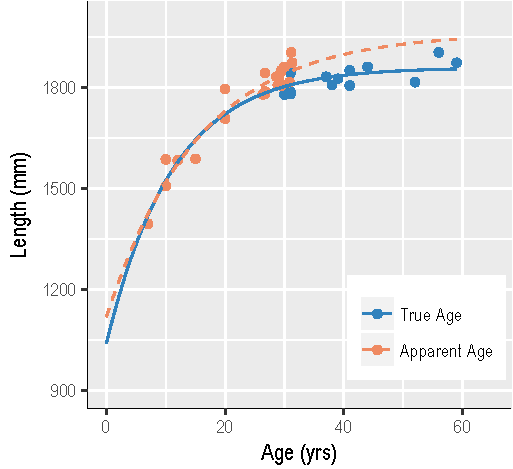
\includegraphics{/Users/alharry/Documents/Manuscripts/age-underestimation/reports/Supplementary material_files/figure-latex/figS1-1} \end{center}

\subsubsection{Facet (b)}\label{facet-b}

Assuming that age underestimation is predominantly a function of length
(Figure 3 b), faster and slower growing individuals would be affected
differently, and growth zones accurate for a variable portion of total
lifespan. To illustrate this, the von Bertalanffy growth curve for New
Zealand porbeagle sharks was plotted with \emph{k} varying from 0.05 to
0.175 in increments of 0.025. Ages \textgreater{} 88\% of \(L_\infty\)
(based on the analysis in Figure 3b) are shaded differently to show the
most likely ages affected.

\begin{center}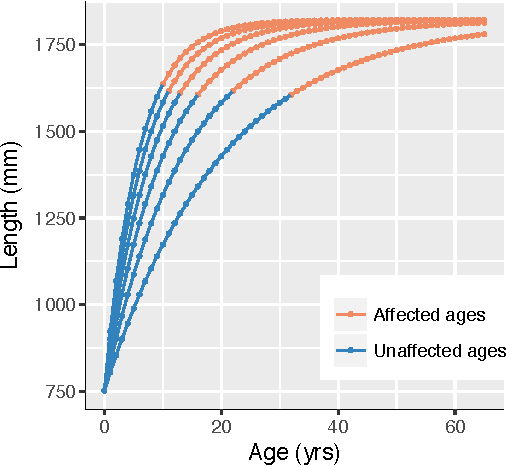
\includegraphics{/Users/alharry/Documents/Manuscripts/age-underestimation/reports/Supplementary material_files/figure-latex/figS2-1} \end{center}

\subsubsection{Facet (c)}\label{facet-c}

The underestimation of age may have important implications for the
estimation of mortality, particularly if using age-structured models
that are fit to length-at-age data. If not accounted for, this apparent
`loss of age structure' would be indistinguishable from fishing
mortality, potentially resulting in erroneous conclusions being drawn
about the total mortality experienced by the population. To illustrate
this, 300 individuals were randomly sampled from a simulated population
as described above, and true and apparent age structures plotted for
comparison.

\begin{center}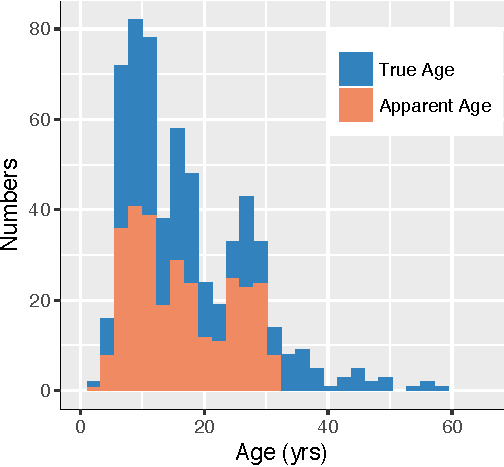
\includegraphics{/Users/alharry/Documents/Manuscripts/age-underestimation/reports/Supplementary material_files/figure-latex/figS3-1} \end{center}

\subsubsection{Facet (d)}\label{facet-d}

Bias in parameters such as longevity may also influence demographic
analyses. Direct estimates of natural mortality, \emph{M} are typically
unavailable for fish stocks, so this quantity is often calculated using
life history invariant relationships based on longevity. To illustrate
this, a simple demographic analysis using an age structured Leslie
matrix (Caswell 2001) was undertaken where \emph{M} was again
approximated using the Hoenig method above as \(M = 4.3/A_{Max}\). The
projection matrix, \textbf{A}, was given by: \[\begin{bmatrix}
f_0 & f_1 & f_2 & ... & f_{a-1}\\ 
s_1 & 0 & 0 & 0 & 0\\ 
0 & s_2 & 0 & 0 & 0\\ 
0 & 0 & ... & 0 & 0\\ 
0 & 0 & 0 & s_{a-1}& 0
\end{bmatrix}\] where \(s_a\) and \(f_a\) are age-specific values of
survival and fecundity in a birth-pulse population with a pre-breeding
census, and where annual survival is assumed to be constant and
calculated as \(s_a = e^{-M}\). Age-specific fecundity (females only)
was calculated as \(f_a = F_a s_a\), where the number of female pups at
any given age, \(F_a\) is calculated as \[ F_a = \begin{cases}
 & \text{ if } a<A_{Mat}, \quad 0\\ 
 & \text{ if } a\geq A_{Mat}, \quad F/2/R))) 
\end{cases}\] were \(A_{Mat}\) is age at maturity (plus one year to
account for the the duration of the reproductive cycle), and where
\emph{F} is average fecundity, divided by the sex ratio, and frequency
of reproduction in years, \emph{R}. The instantaneous rate of population
growth, \(\lambda\) was obtained as the real component of the dominant
eigenvalue of \textbf{A}. Population doubling time was then calculated
as \[t_2 = log_{\lambda}2\] The Leslie matrix was run with both the true
longevity and appararent longevity of New Zealand porbeagle sharks
(Table S1) while keeping all other parameters the same. To illustrate
the sensitivity of the model to changes in maximum age, relative
population size was projected forward exponentially for 22 years (the
population doubling time when using the apparent longevity).

\begin{center}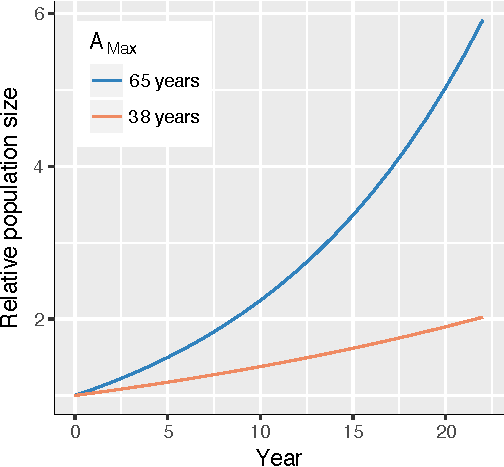
\includegraphics{/Users/alharry/Documents/Manuscripts/age-underestimation/reports/Supplementary material_files/figure-latex/figS4-1} \end{center}

\subsection*{References}\label{references}
\addcontentsline{toc}{subsection}{References}

\hypertarget{refs}{}
\hypertarget{ref-caswell_matrix_2001}{}
Caswell, H. (2001) \emph{Matrix population models. Construction,
analysis, and interpretation}, 2nd Edition. Sinauer Associates, Inc.,
Sutherland, MA.

\hypertarget{ref-francis_reproduction_2000}{}
Francis, M. and Stevens, J. (2000) Reproduction, embryonic development,
and growth of the porbeagle shark, \emph{Lamna nasus} , in the southwest
Pacific Ocean. \emph{Fishery Bulletin} \textbf{98}, 41--63.

\hypertarget{ref-francis_age_2007}{}
Francis, M.P., Campana, S.E. and Jones, C.M. (2007) Age under-estimation
in New Zealand porbeagle sharks (\emph{Lamna nasus}): Is there an upper
limit to ages that can be determined from shark vertebrae? \emph{Marine
and Freshwater Research} \textbf{58}, 10--23.
doi:\href{https://doi.org/10.1071/MF06069}{10.1071/MF06069}.

\hypertarget{ref-kenchington_natural_2014}{}
Kenchington, T.J. (2014) Natural mortality estimators for
information-limited fisheries. \emph{Fish and Fisheries} \textbf{15},
533--562.
doi:\href{https://doi.org/10.1111/faf.12027}{10.1111/faf.12027}.


\end{document}
